\documentclass[tikz,border=5pt]{standalone}
\usepackage{pgfplots}
\usepgfplotslibrary{groupplots,fillbetween}

\pgfplotsset{compat=1.18}

\begin{document}
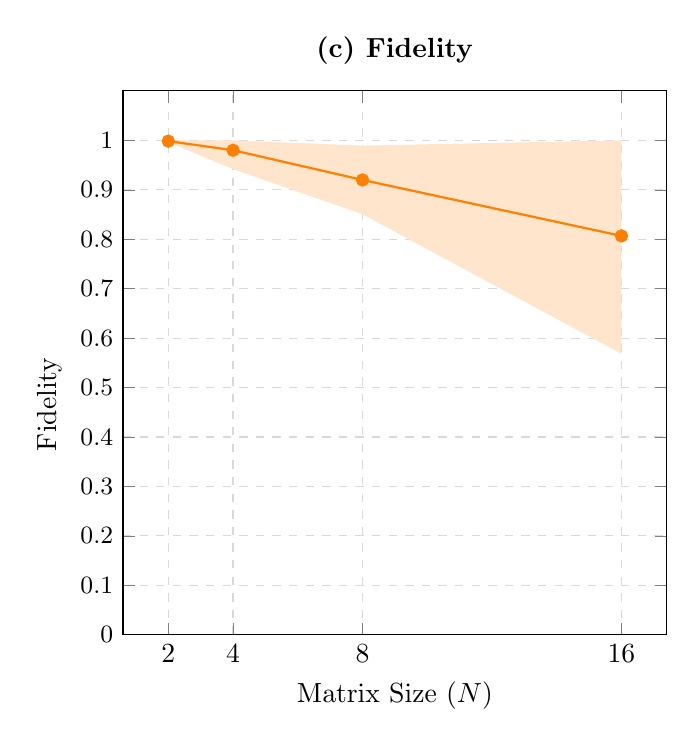
\begin{tikzpicture}
\begin{axis}[
    width=0.7\columnwidth,
    height=0.7\columnwidth,
    grid=major,
    grid style={dashed, gray!30},
    xlabel={Matrix Size ($N$)},
    xtick = {2,4,8,16},
    ylabel={Fidelity},
    ylabel style ={xshift=-15pt},
    title={\textbf{(c) Fidelity}},
    ymin=0,
    ytick={0,0.1,0.2,0.3,0.4,0.5,0.6,0.7,0.8,0.9,1},
    yticklabel style={font=\small},
]
\addplot[name path=upper,draw=none] coordinates { (2, 1.0000) (4, 1.0000) (8, 0.9895) (16, 1.0000) };
\addplot[name path=lower,draw=none] coordinates { (2, 0.9962) (4, 0.9420) (8, 0.8506) (16, 0.5683) };
\addplot[orange!20] fill between[of=upper and lower];
\addplot[orange,thick,mark=*] coordinates { (2, 0.9985) (4, 0.9801) (8, 0.9200) (16, 0.8068) };
\end{axis}
\end{tikzpicture}
\end{document}